The reducible backgrounds estimated with the methods described in the previous 
sections are validated by comparing observed data to 
predicted background after various kinematic requirements. 
The next sections will validate 
the MC template method used to estimate the charge flip and the FNP lepton 
background, and the matrix method used to estimate the FNP lepton background.



\subsection*{Data/MC comparisons}

The overall level of agreement obtained by the matrix method
can be seen in different channels in Fig~\ref{fig:distributions_summary}. 
The distributions of several variables are shown on Fig~\ref{fig:Bkg_distribs} for an inclusive same-sign leptons selection
after various requirements on the number of jets and $b$-jets.
These distributions illustrate that the data are described by the prediction 
within uncertainties. 
The apparent disagreement 
for \meff\ above 1 TeV~in Figure~\ref{fig:VRmeff2} is covered by the large 
theory uncertainty for the diboson background, which is not shown 
but amounts to about 30\% for \meff\ above 1 \TeV. 
%Similar distributions for the other main variables can be found in 
%Appendix~\ref{chap:app.bkg.val}.
To avoid the presence of signal in the tails of these distributions, 
events belonging to any of the signal regions are vetoed 
both in data and for the predicted backgrounds. 

\begin{figure}[t!]
\centering
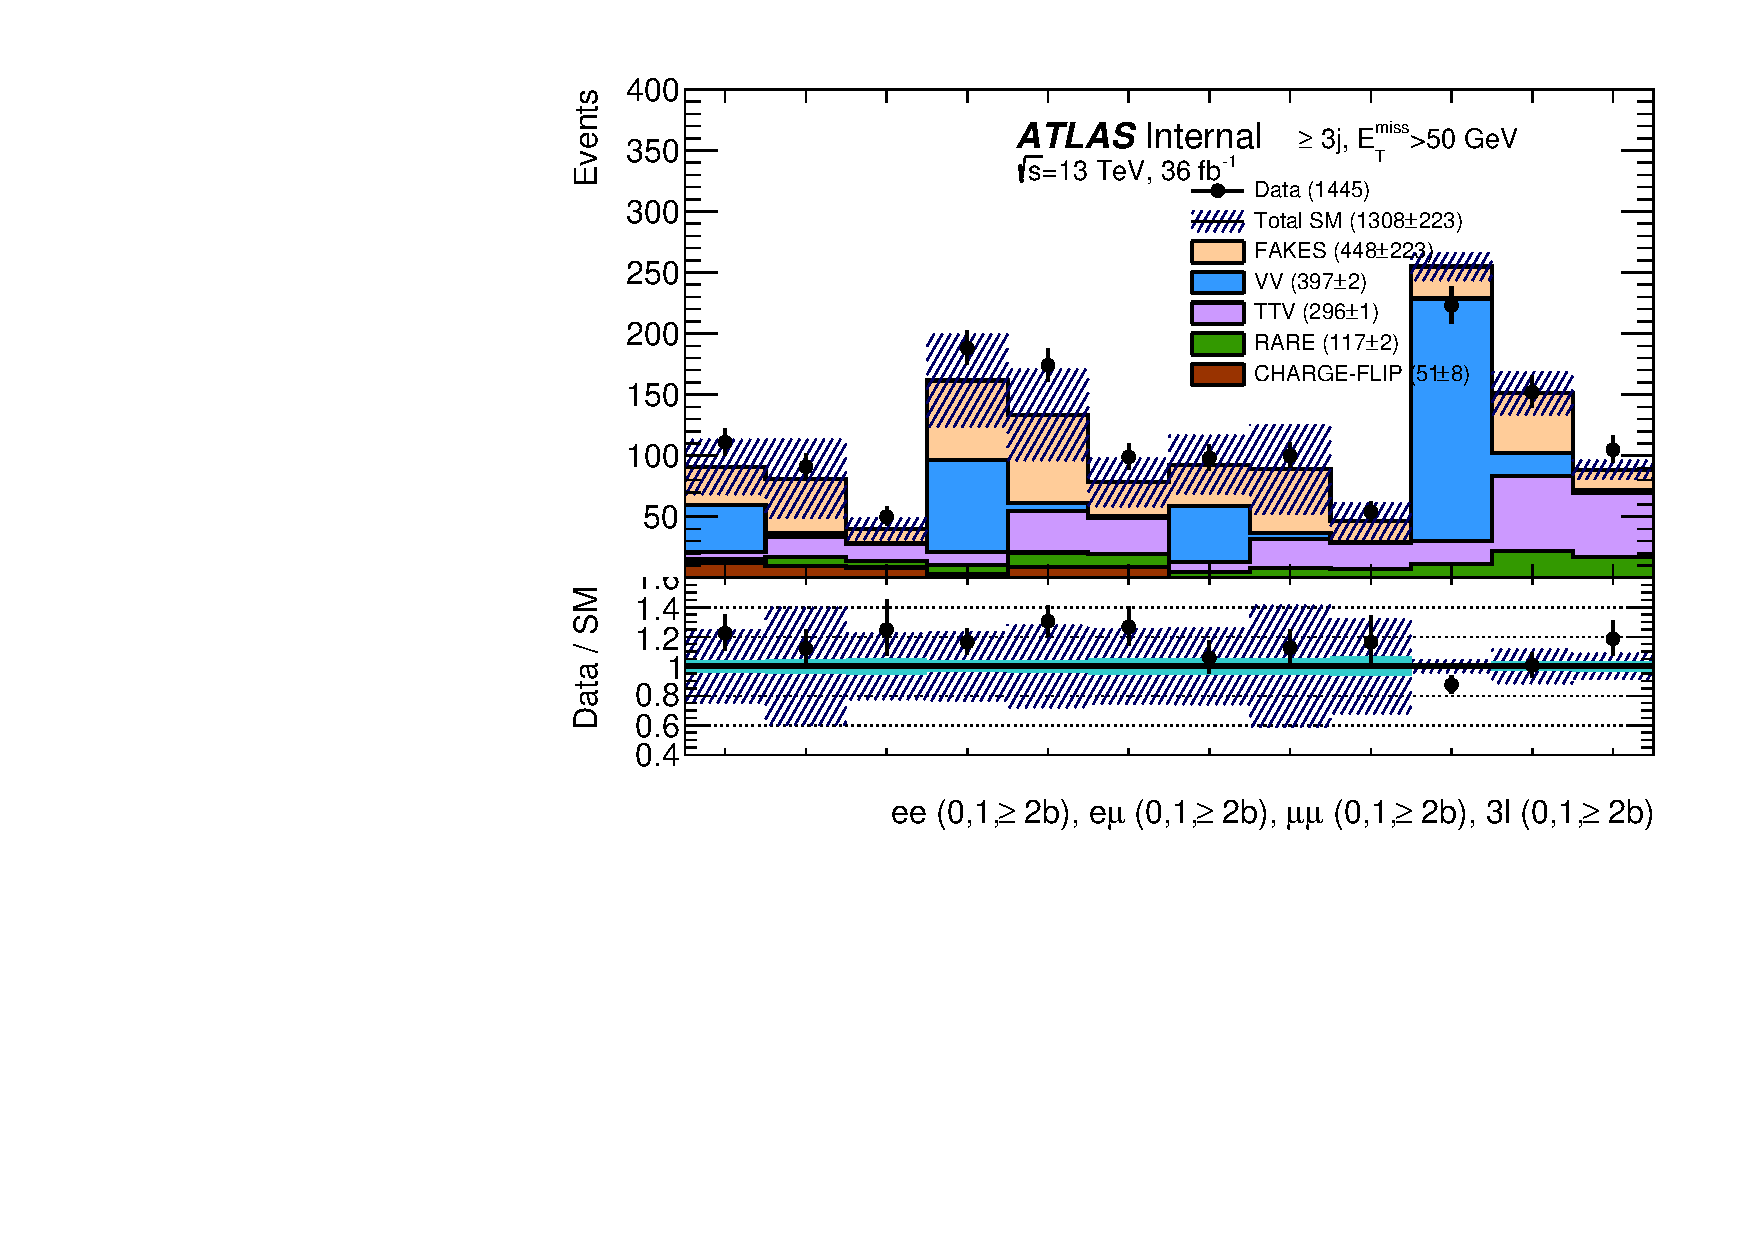
\includegraphics[width=0.8\textwidth]{ALL_MET50}
\caption{Summarized level of agreement between observed data (2015+2016, 36.5 \ifb) and expected SM+detector backgrounds 
for events with $\ge 2$ same-sign leptons ($\pt>20 \GeV$), $\met>50 \GeV$ and $\ge 3$ jets ($\pt>40 \GeV$), 
split as function of the lepton flavours and the number of $b$-tagged jets. 
Uncertainties include statistical sources, as well as systematic uncertainties for the data-driven backgrounds; 
for illustration, statistical uncertainties alone are shown in the light-colored error bands in the ratio plots. 
Events belonging to any of the signal regions are rejected, both in data and MC. 
}
\label{fig:distributions_summary}
\end{figure} 

\begin{figure}[th!]
\centering
\begin{subfigure}[t]{0.49\textwidth}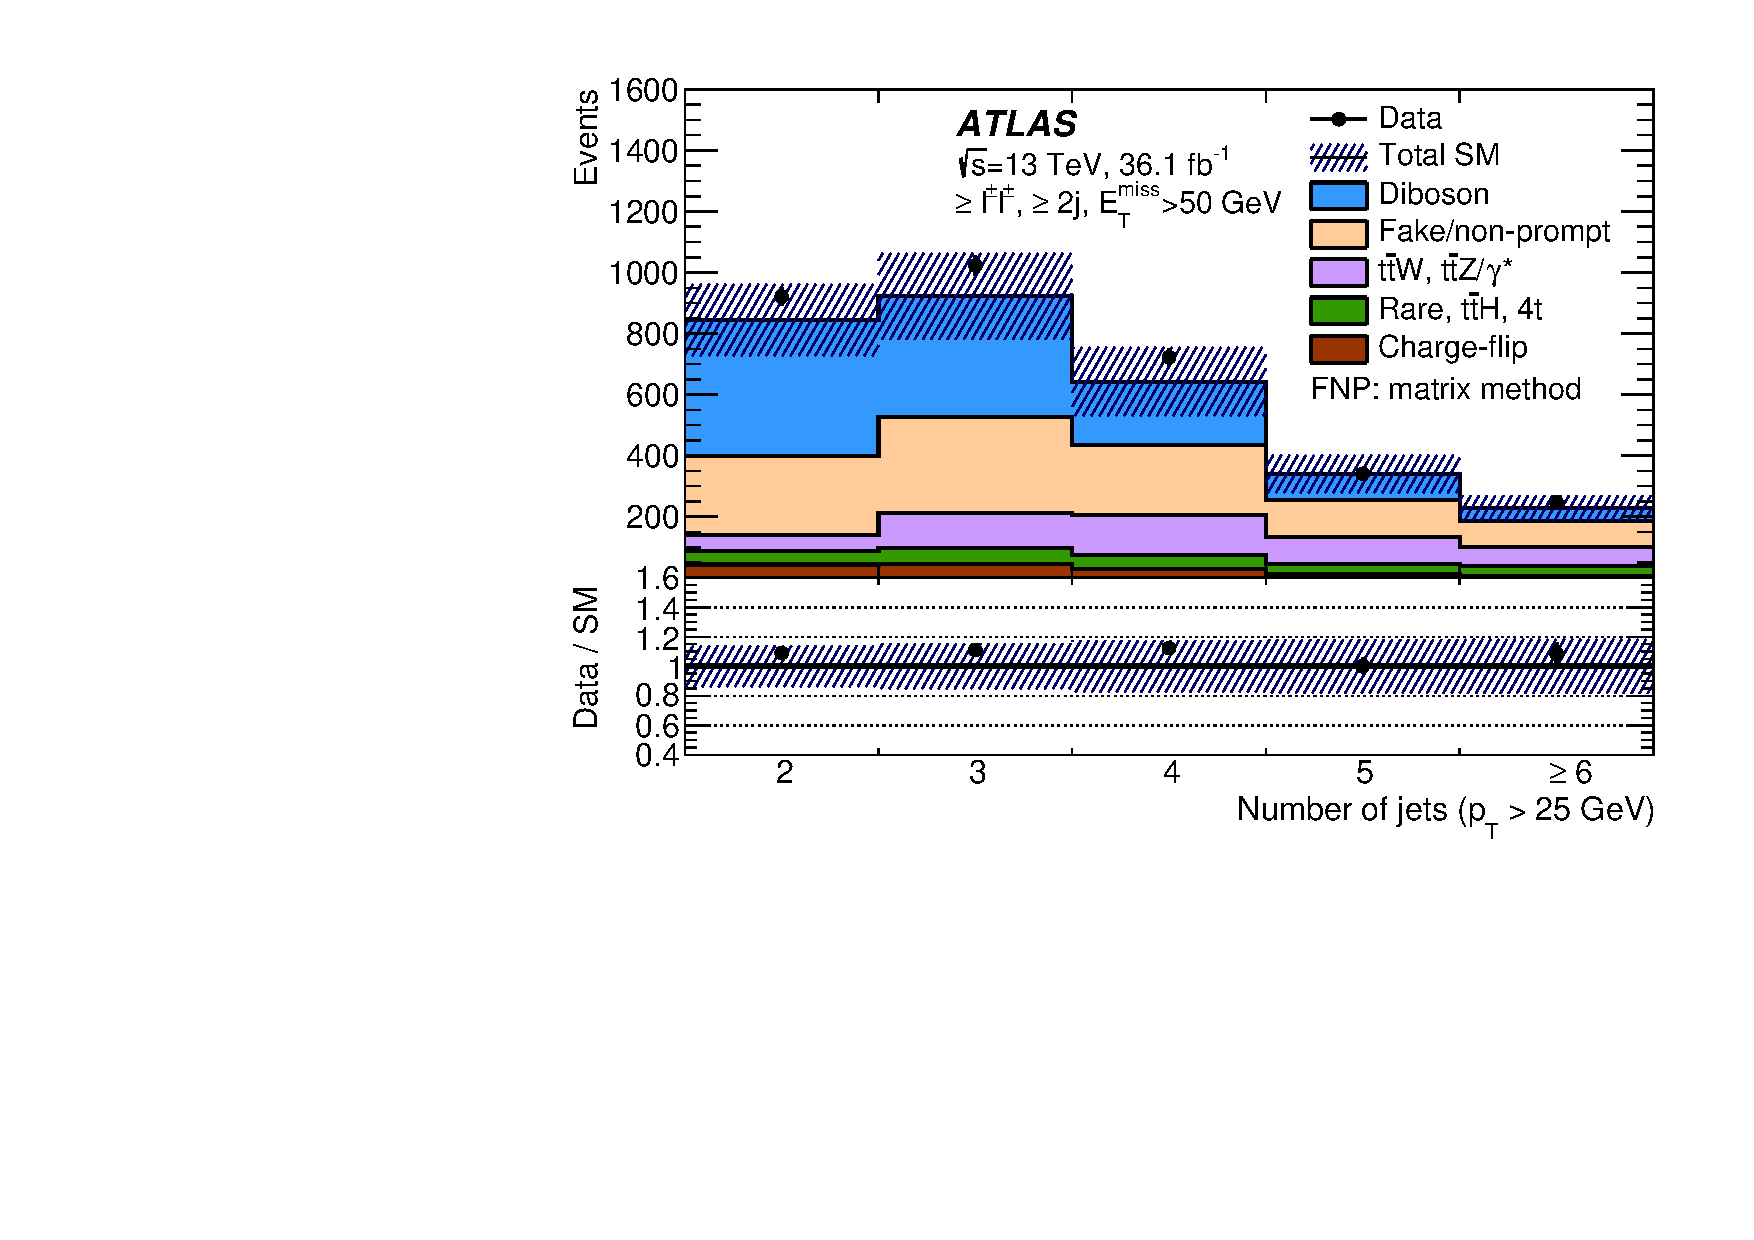
\includegraphics[width=\textwidth]{PAPER_DILEP_2JMET50_njets25}\caption{}\label{fig:VRnj}\end{subfigure}
\begin{subfigure}[t]{0.49\textwidth}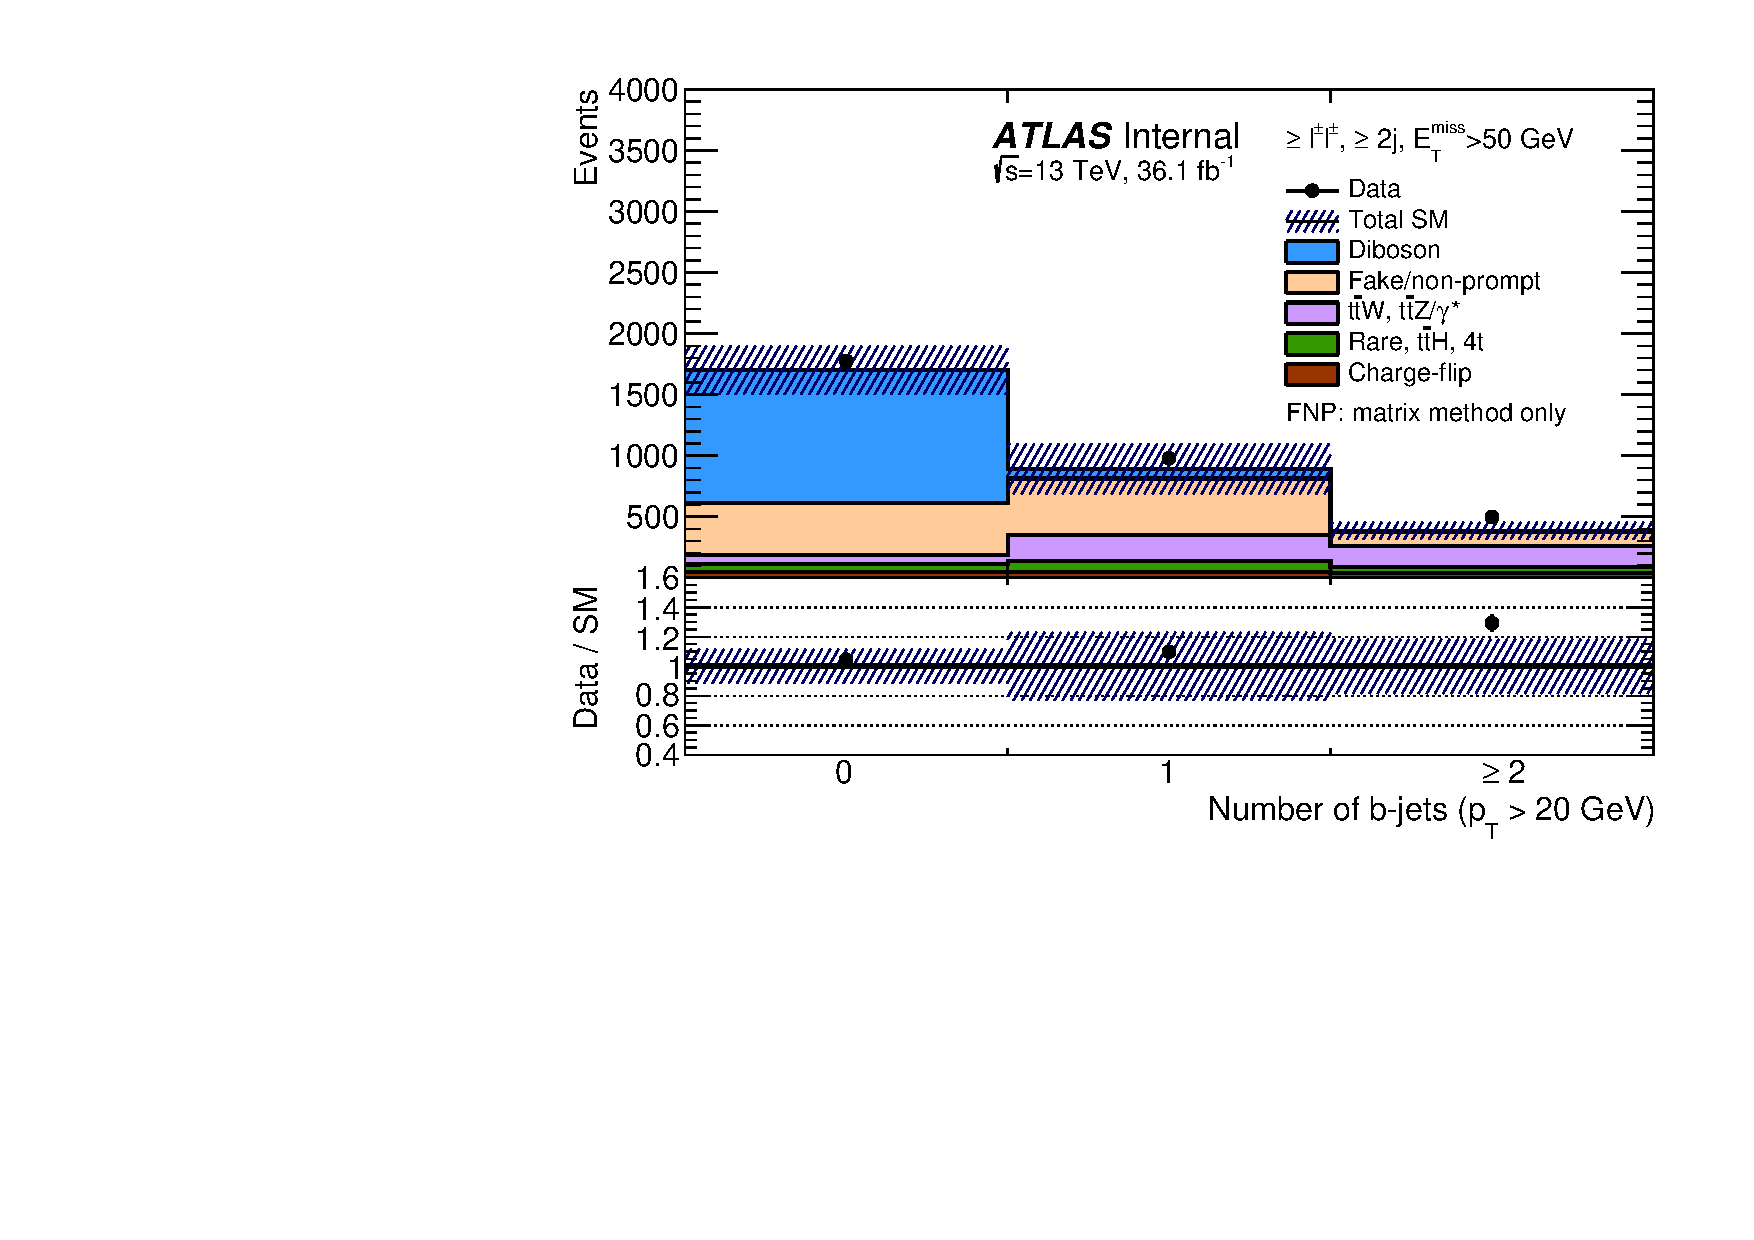
\includegraphics[width=\textwidth]{PAPER_DILEP_2JMET50_nbjets}\caption{}\label{fig:VRnb}\end{subfigure}
\begin{subfigure}[t]{0.49\textwidth}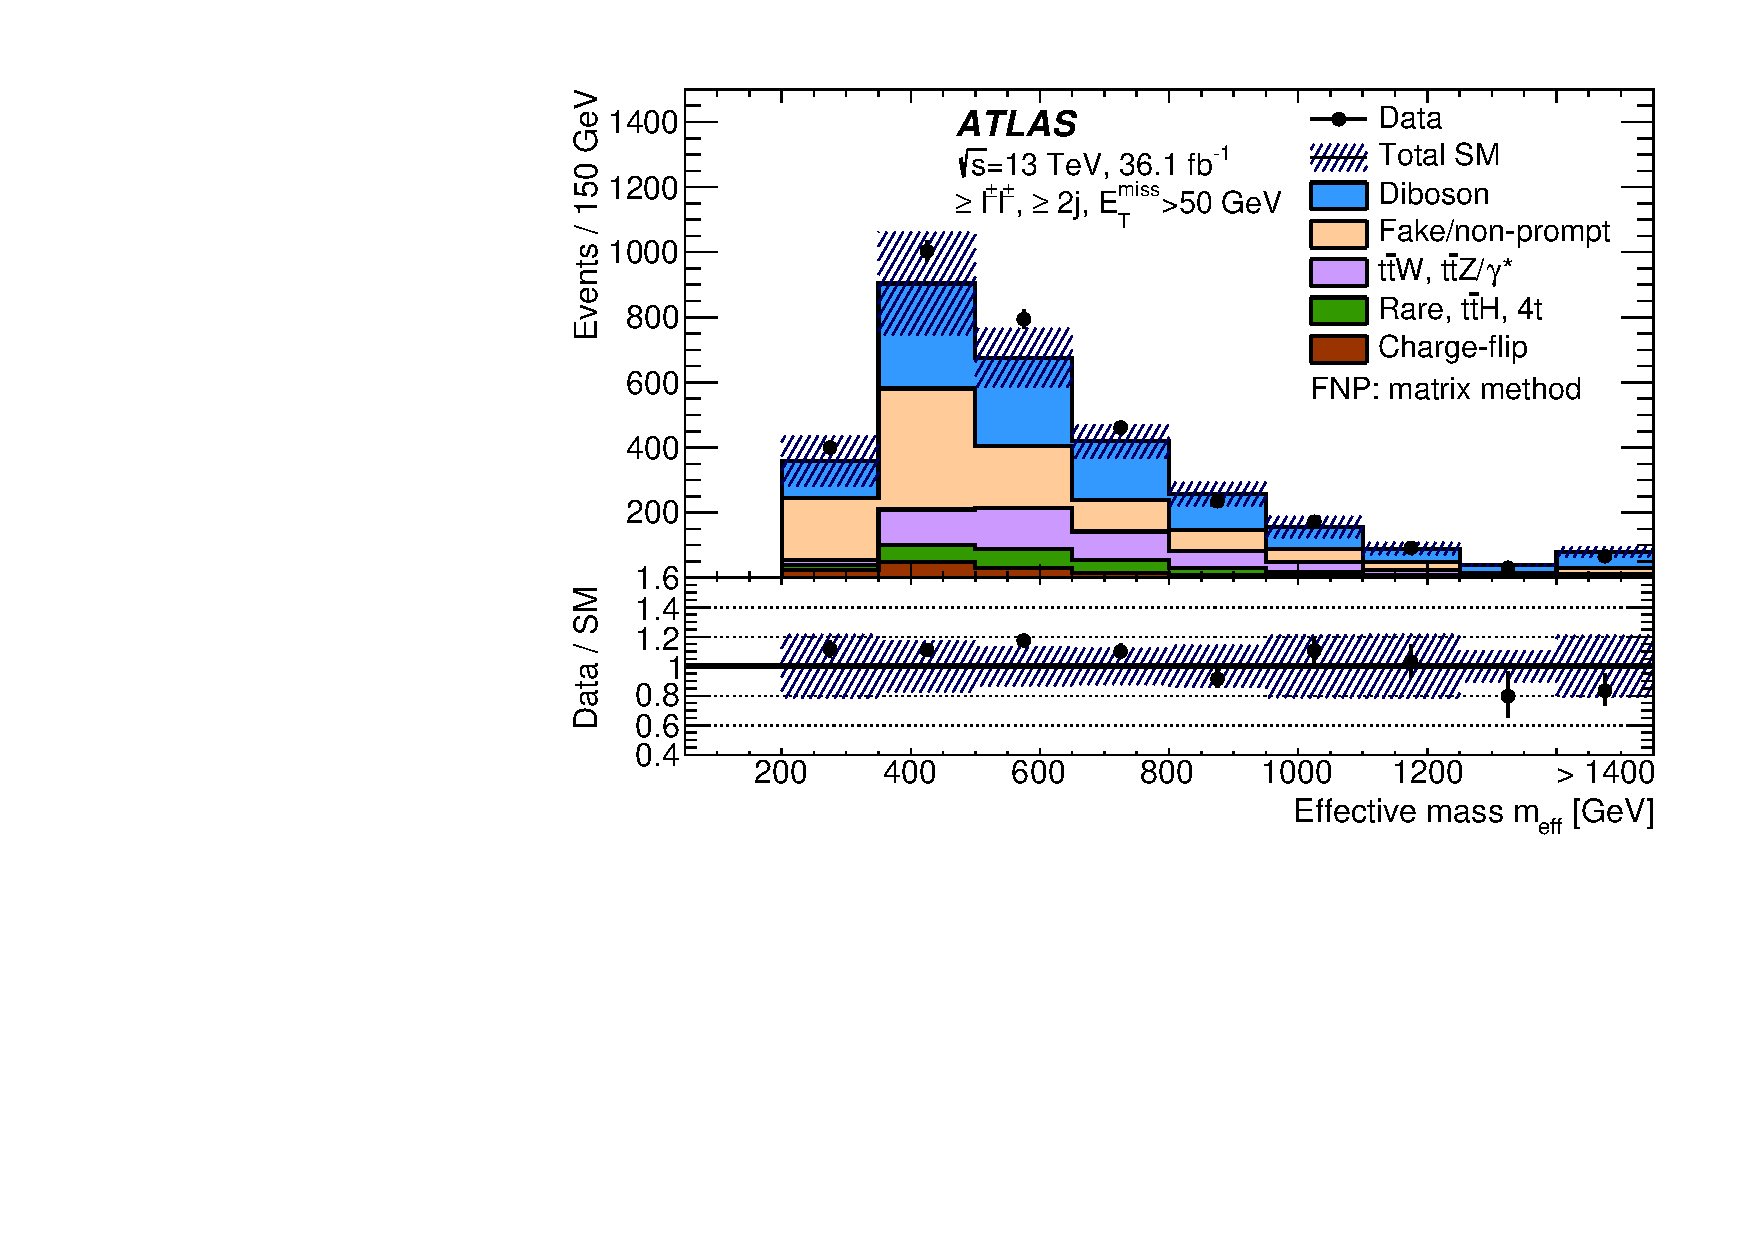
\includegraphics[width=\textwidth]{PAPER_DILEP_2JMET50_meff}\caption{}\label{fig:VRmeff1}\end{subfigure}
\begin{subfigure}[t]{0.49\textwidth}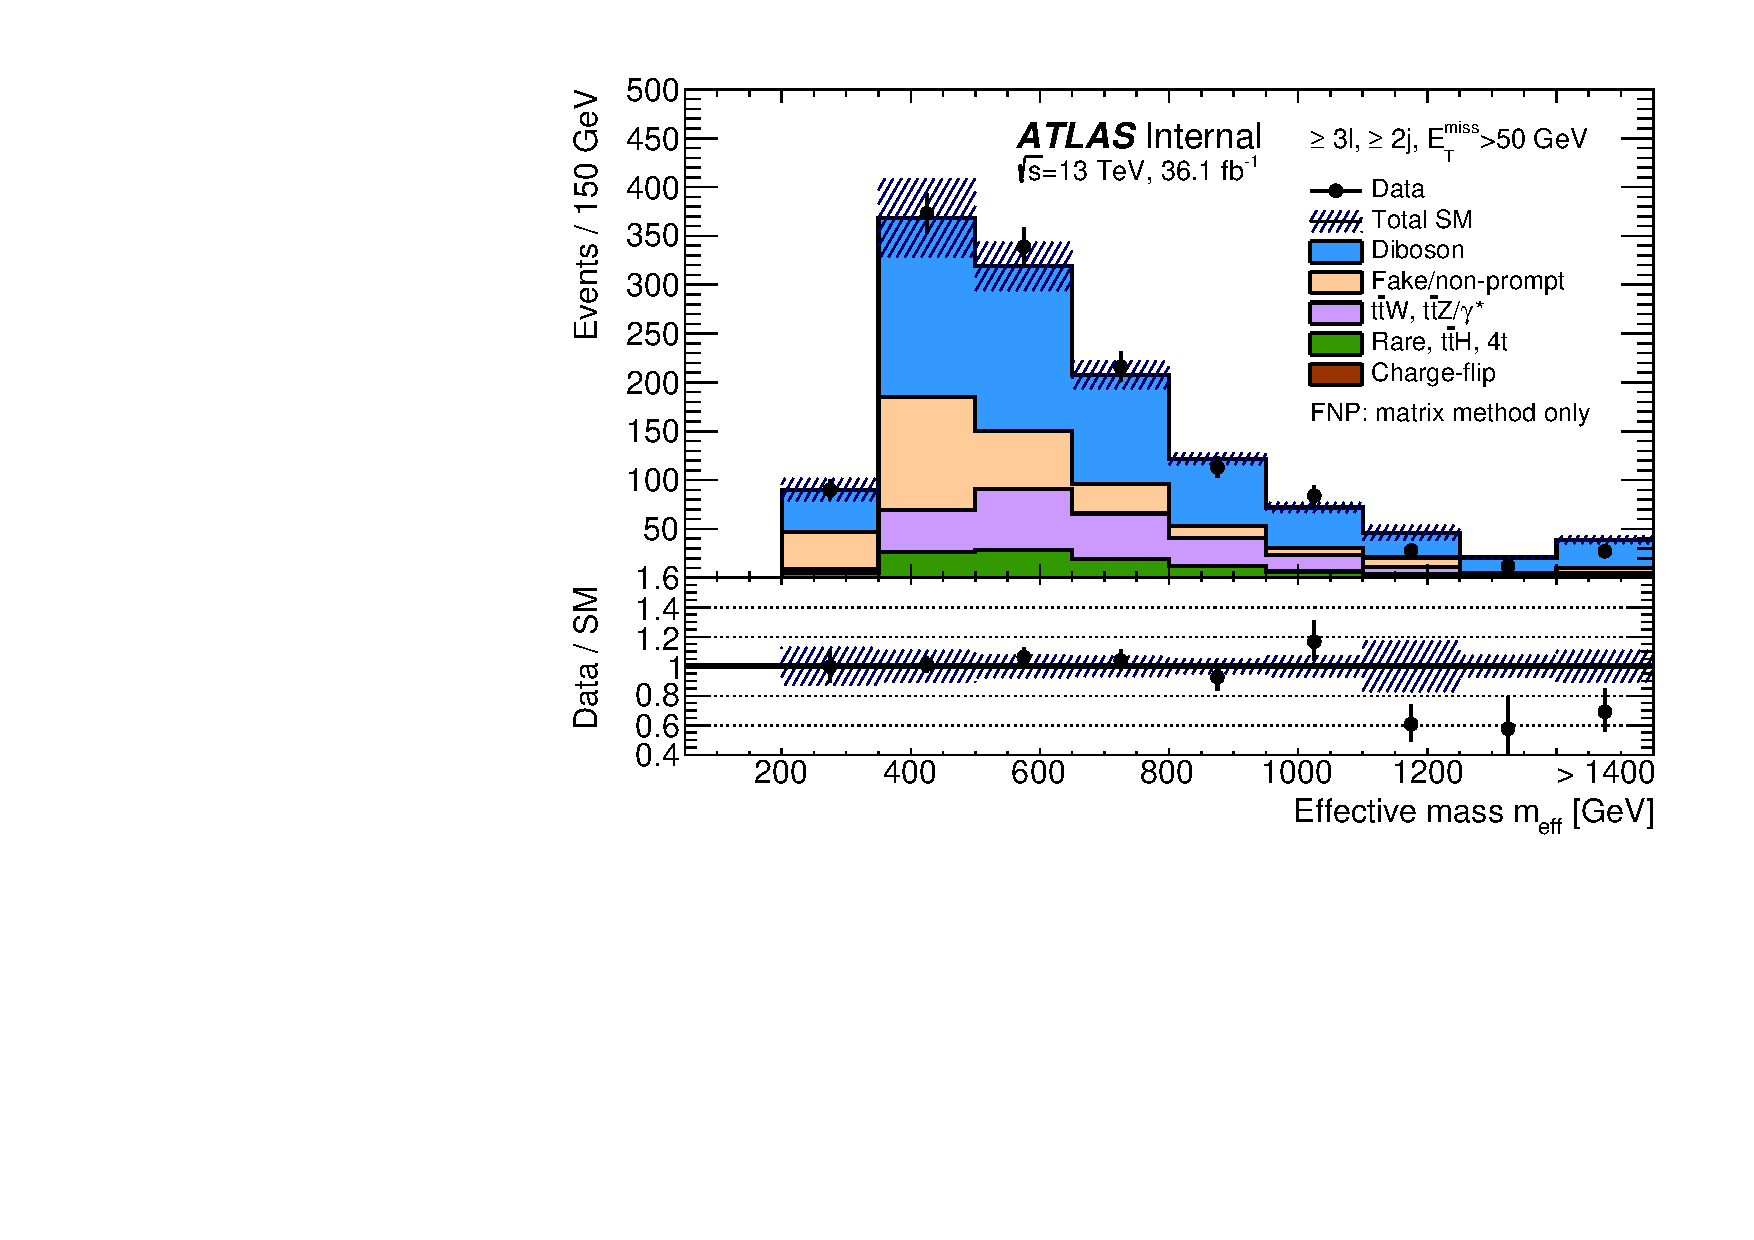
\includegraphics[width=\textwidth]{PAPER_TRILEP_2JMET50_meff}\caption{}\label{fig:VRmeff2}\end{subfigure}
\caption{
Distributions of (a) the number of jets, (b) the number of $b$-tagged jets and (c), (d) the effective mass. The distributions are made 
after requiring at least two jets ($\pT>40 \GeV$) and $\met>50 \GeV$, as well as at least two same-sign leptons ((a), (b), (c)) 
or three leptons (d). The uncertainty bands include the statistical uncertainties for the background prediction as well as the 
systematic uncertainties for fake- or non-prompt-lepton backgrounds (using the matrix method) and charge-flip electrons. Not included
are theoretical uncertainties in the irreducible background contributions.
The rare category is defined in the text.}
\label{fig:Bkg_distribs} 
\end{figure} 


%\subsection*{Validation of the MC template estimates}
%The MC template estimates are validated by checking the agreement between 
%observed data and prediction in different kinematic selections with 
%distributions that were not used in the MC fit to data.
%Some of these distributions are shown in Figure~\ref{}.

%\subsection*{Comparison of the MC template and the matrix method}


Figure~\ref{fig:bkg.val.mctVSmxm} shows a comparison between the estimates of the 
MC template method and the matrix method in a loose selection.
Other \met distributions with events satisfying the signal region 
requirements except the \met\ cut are shown in 
Figure~\ref{fig:bkg.val.met} comparing the two methods. 

\begin{figure}[htb!]
\begin{subfigure}[t]{0.49\textwidth}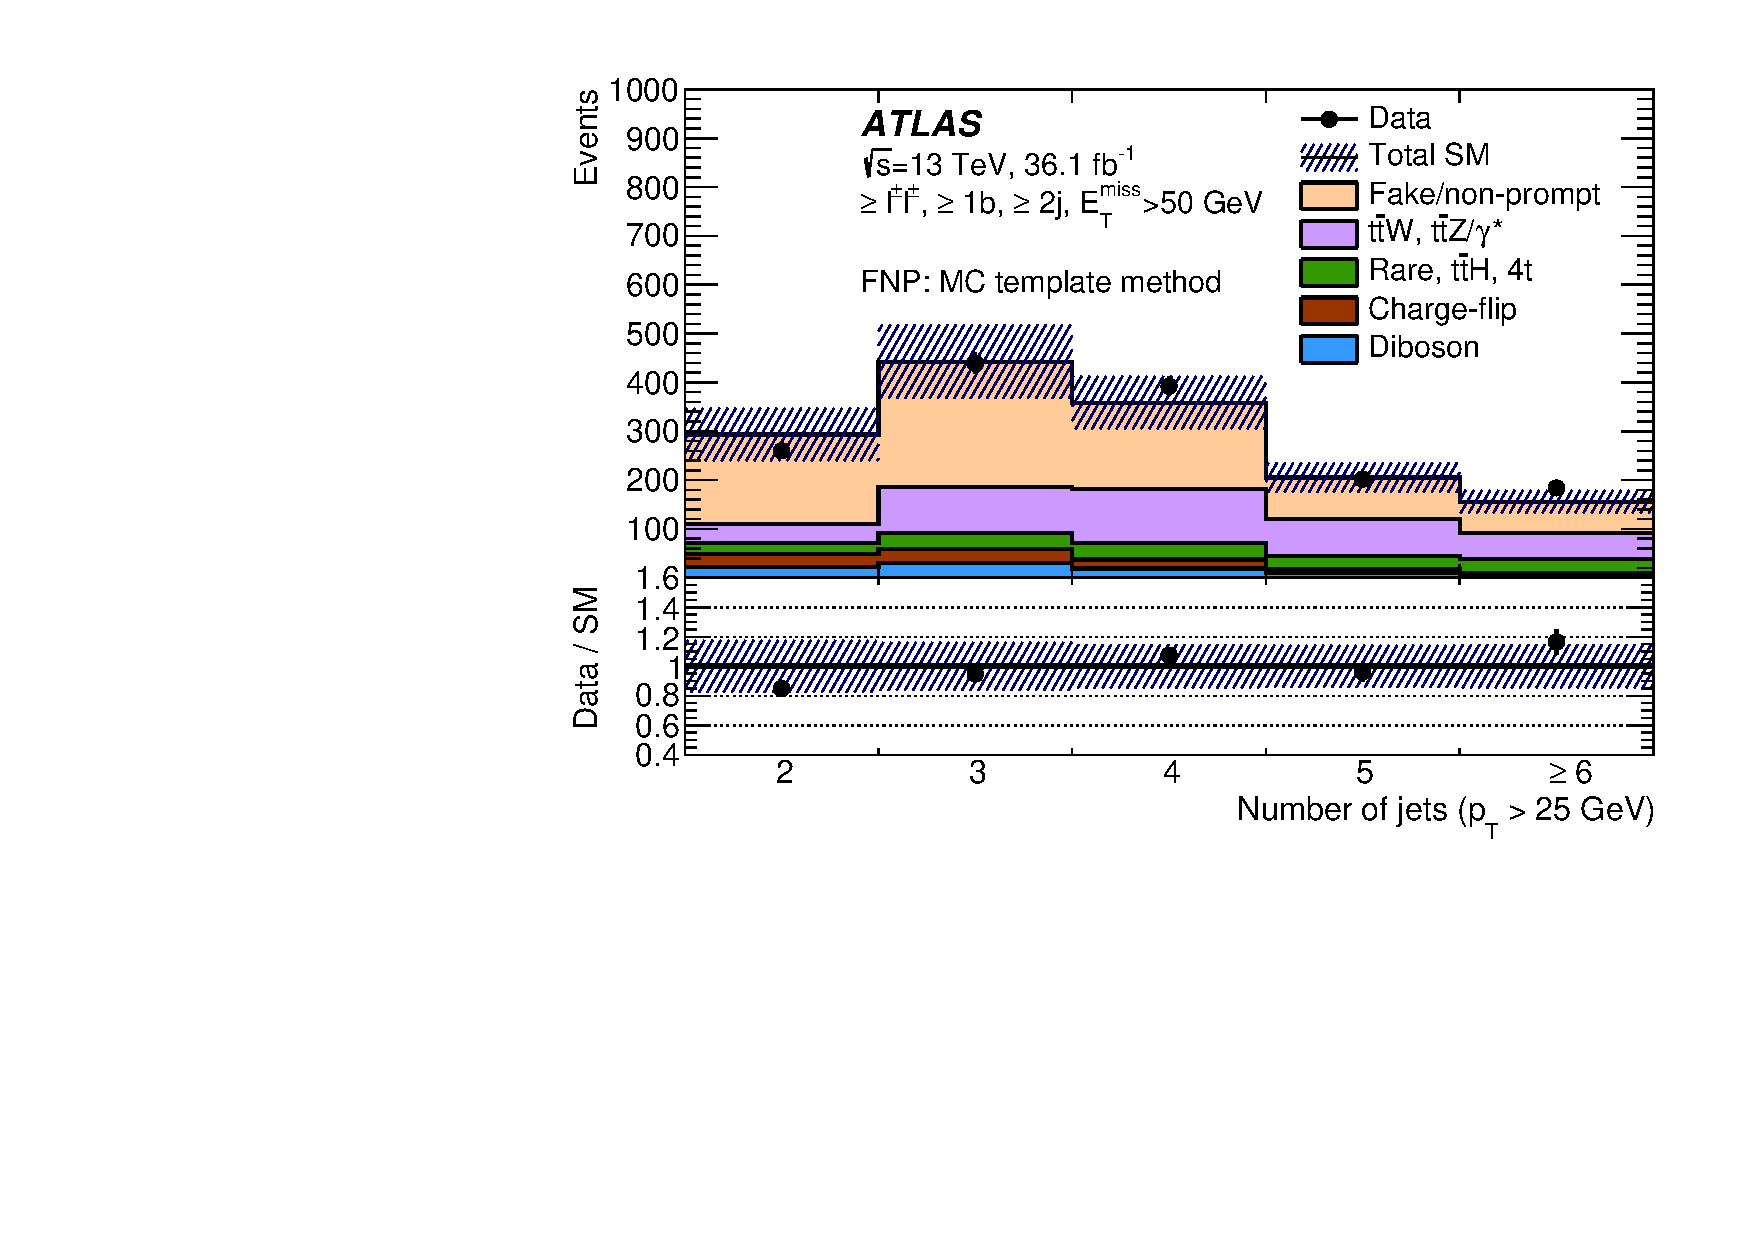
\includegraphics[width=\textwidth]{PAPER_DILEP_1B2JMET50_njets25_template}\caption{}\label{fig:VR1b2j_MxM}\end{subfigure}
\begin{subfigure}[t]{0.49\textwidth}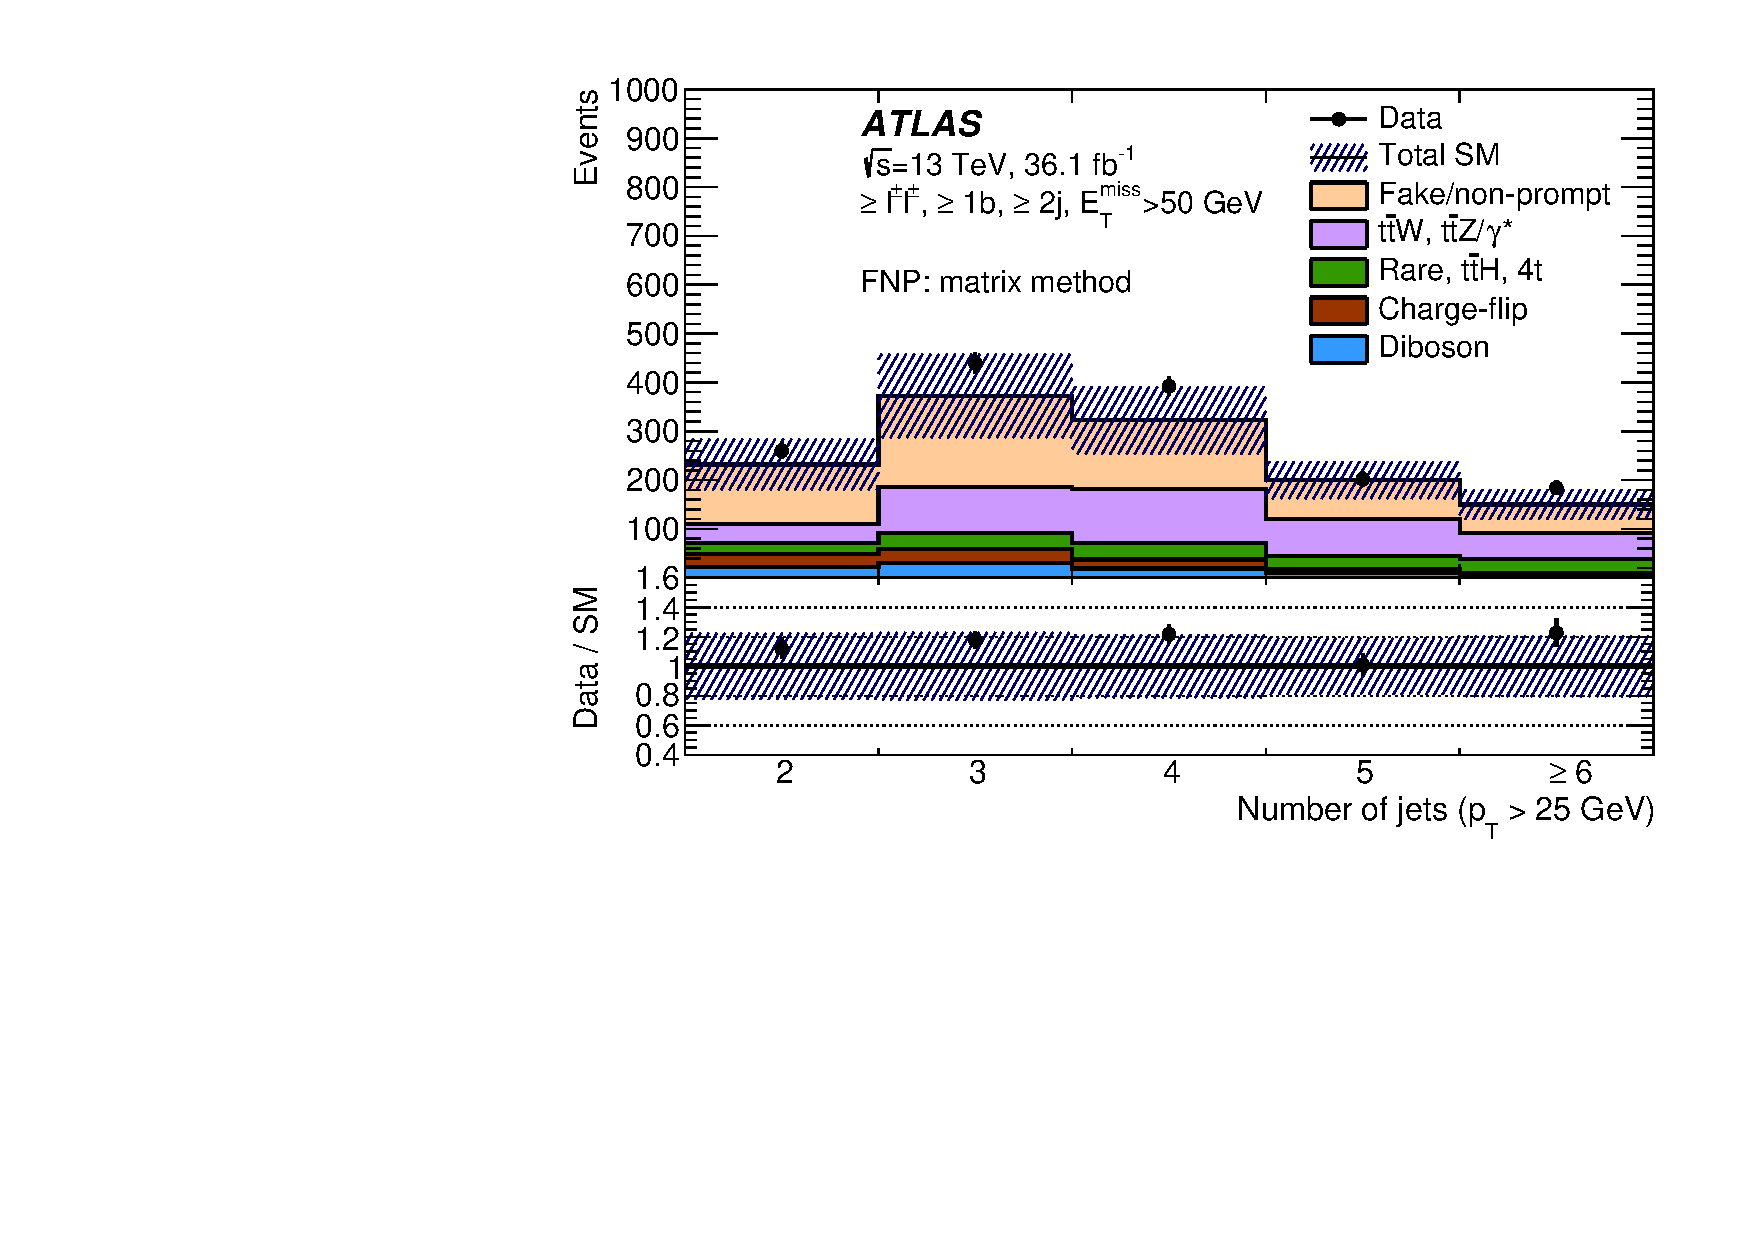
\includegraphics[width=\textwidth]{PAPER_DILEP_1B2JMET50_njets25_matrix}\caption{}\label{fig:VR1b2j_MCT}\end{subfigure}
\caption{
Distributions of the number of jets after requiring at least two jets ($\pT> 40 \GeV$) and $\met> 50 \GeV$, 
as well as at least two same-sign leptons. 
The fake or non-prompt leptons backgrounds are estimated alternatively with the MC template method (\ref{fig:VR1b2j_MCT}) or the matrix method (\ref{fig:VR1b2j_MxM}). 
The uncertainty band includes the statistical uncertainties for the background prediction as well as the
full systematic uncertainties for fake or non-prompt leptons backgrounds or charge-flip electrons. 
The rare category is defined in the text. In both figures, the last bin contains the overflow.
}
\label{fig:bkg.val.mctVSmxm}
\end{figure}


\begin{figure}[htb!]
\begin{subfigure}[t]{0.49\textwidth}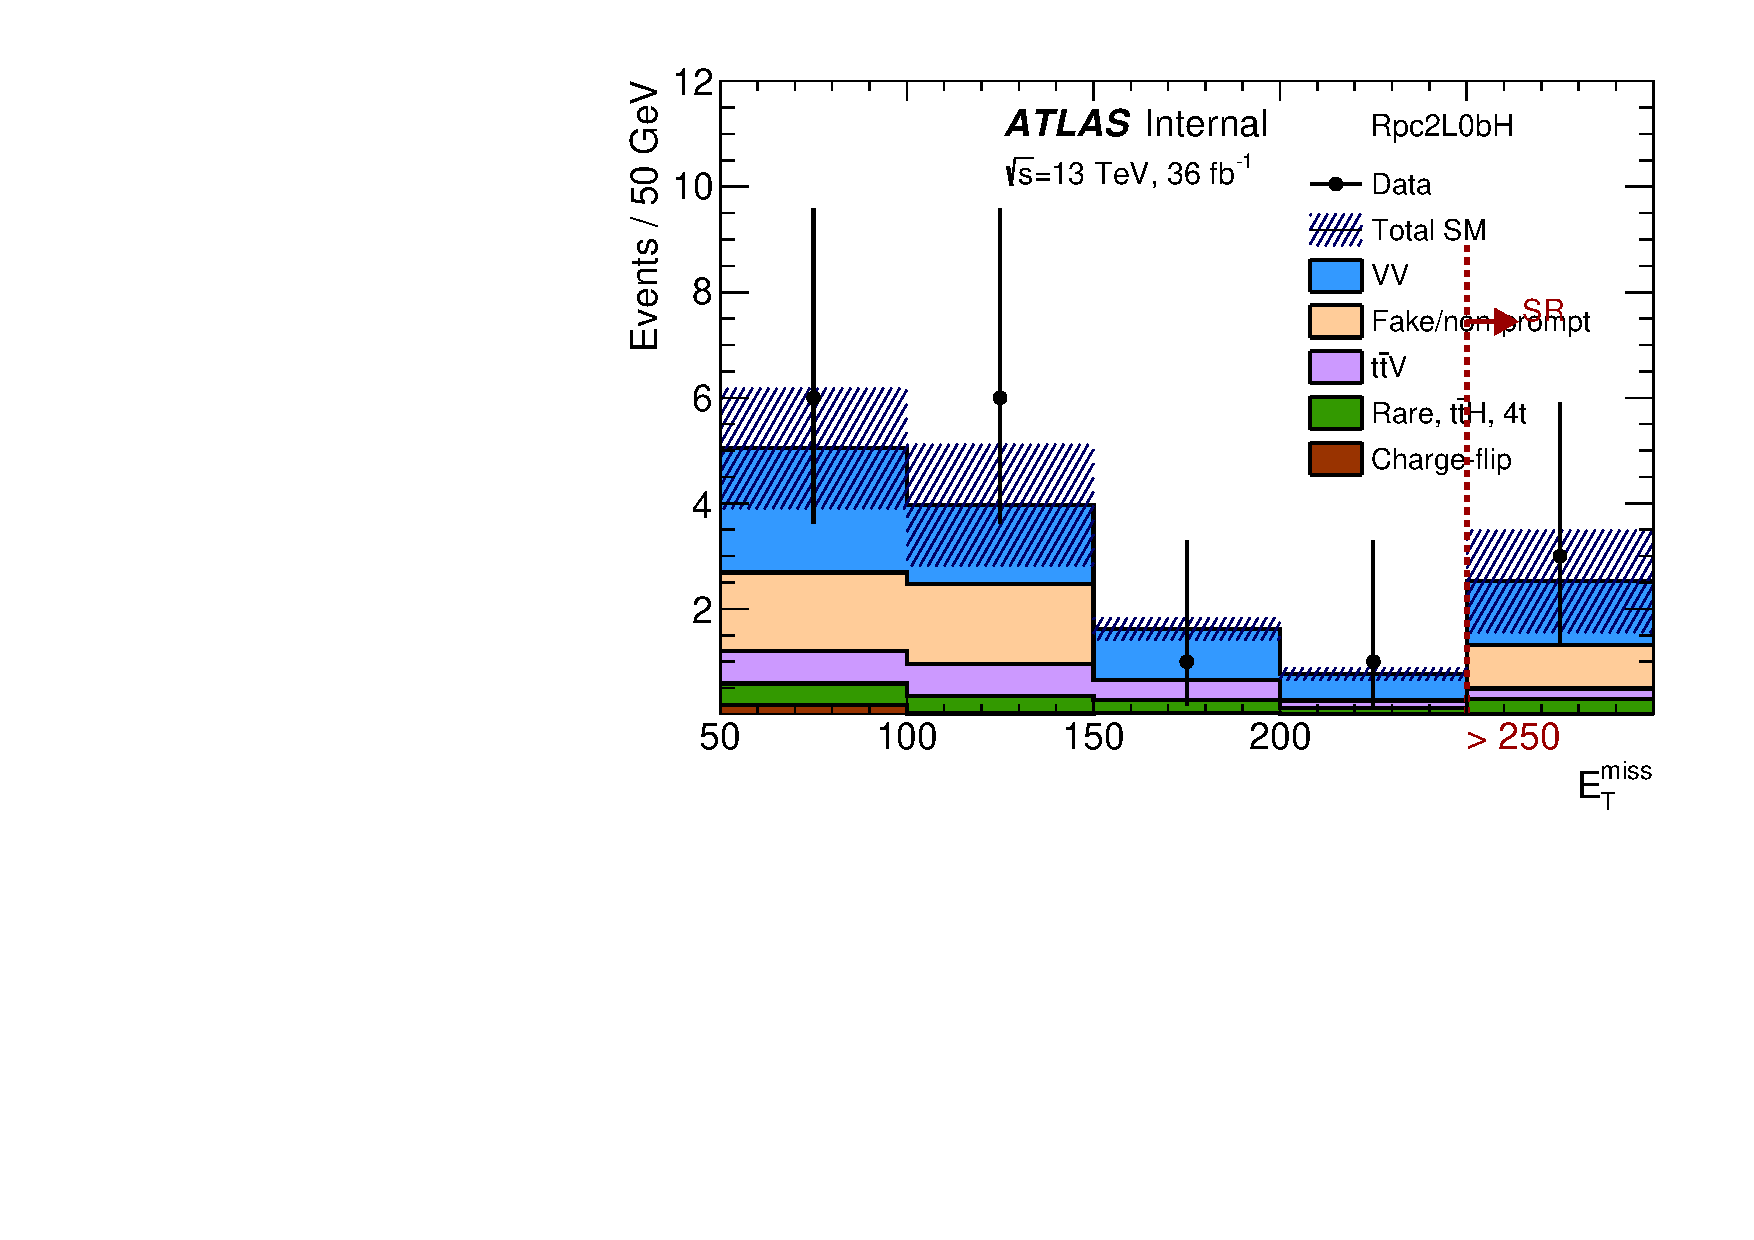
\includegraphics[width=\textwidth]{LooseRpc2L0bH.pdf}\caption{}\label{fig:bkg.val.Rpc2L0bH.MxM}\end{subfigure}
\begin{subfigure}[t]{0.49\textwidth}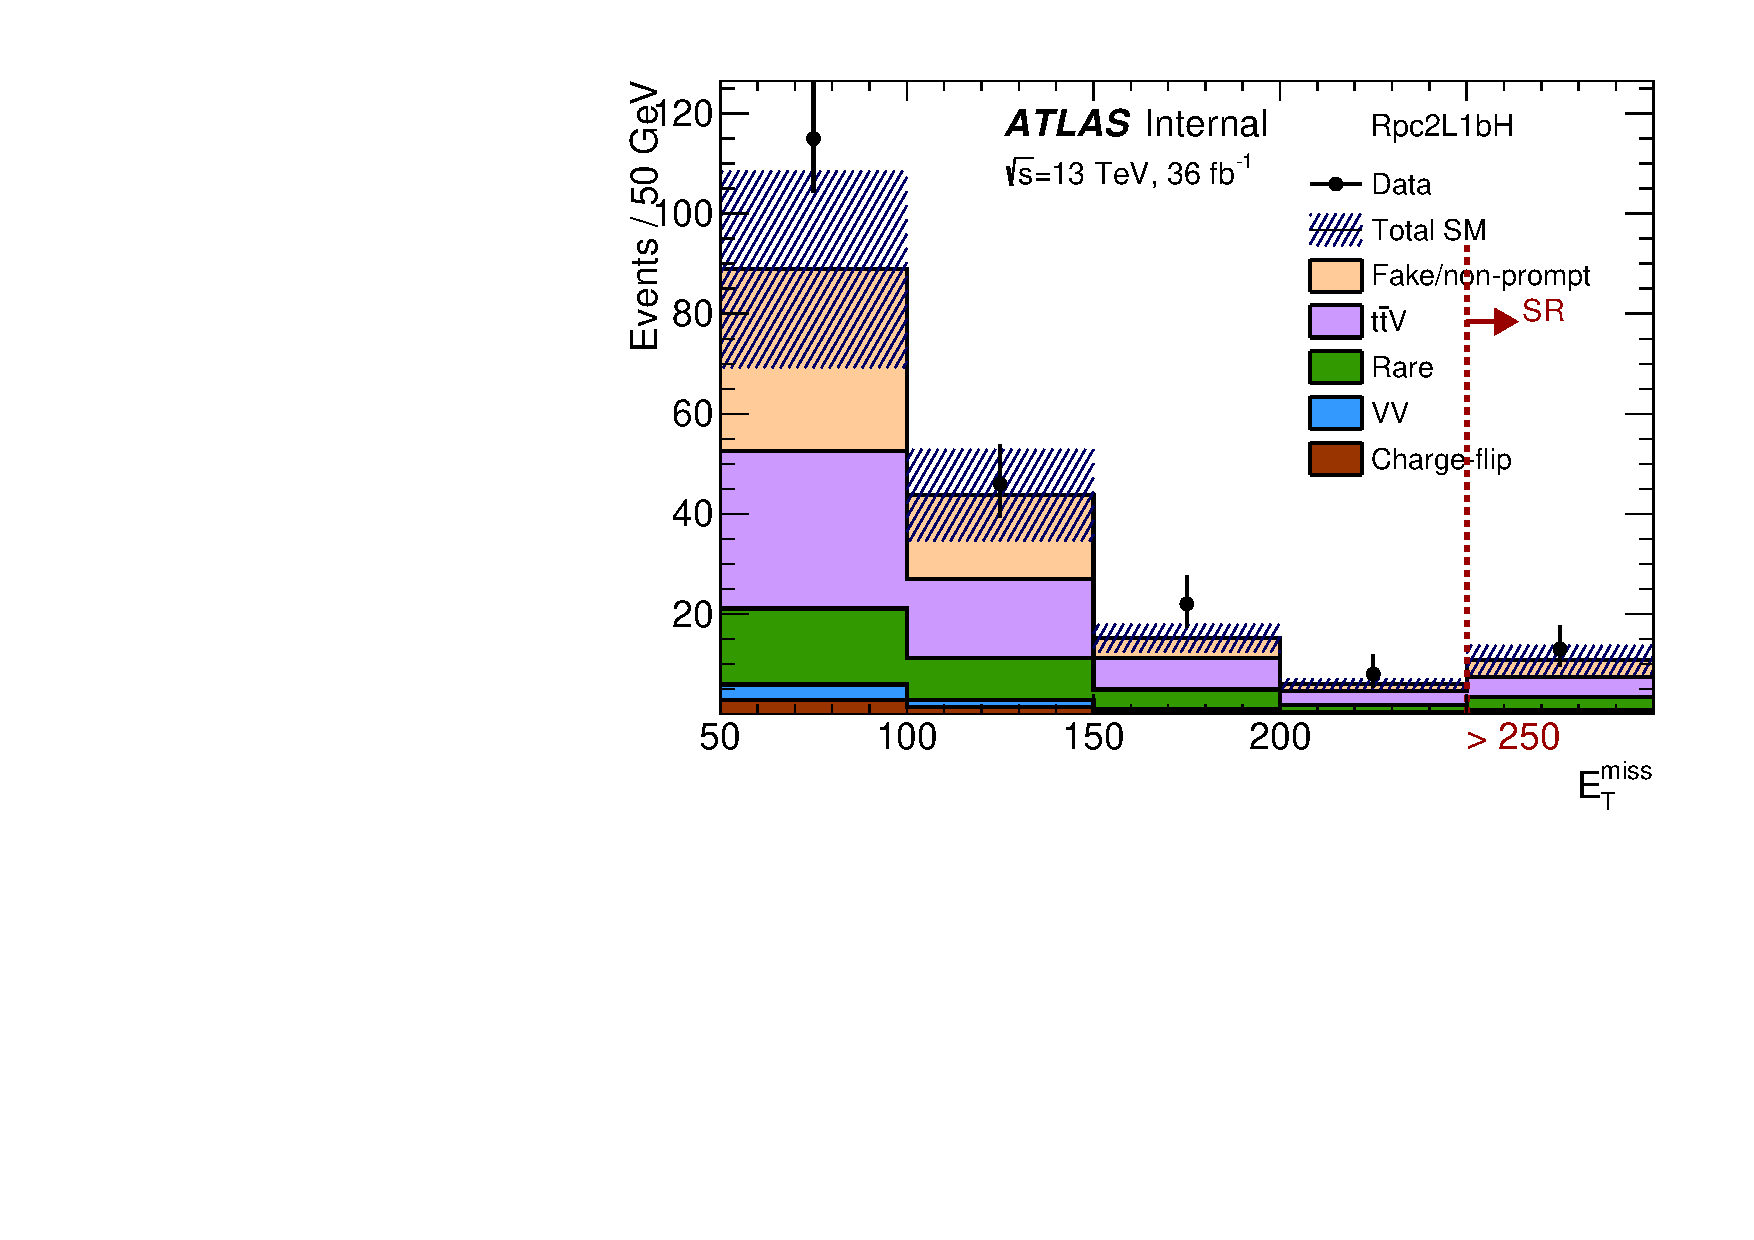
\includegraphics[width=\textwidth]{LooseRpc2L1bH.pdf}\caption{}\label{fig:bkg.val.Rpc2L1bH.MxM}\end{subfigure} \\
\begin{subfigure}[t]{0.49\textwidth}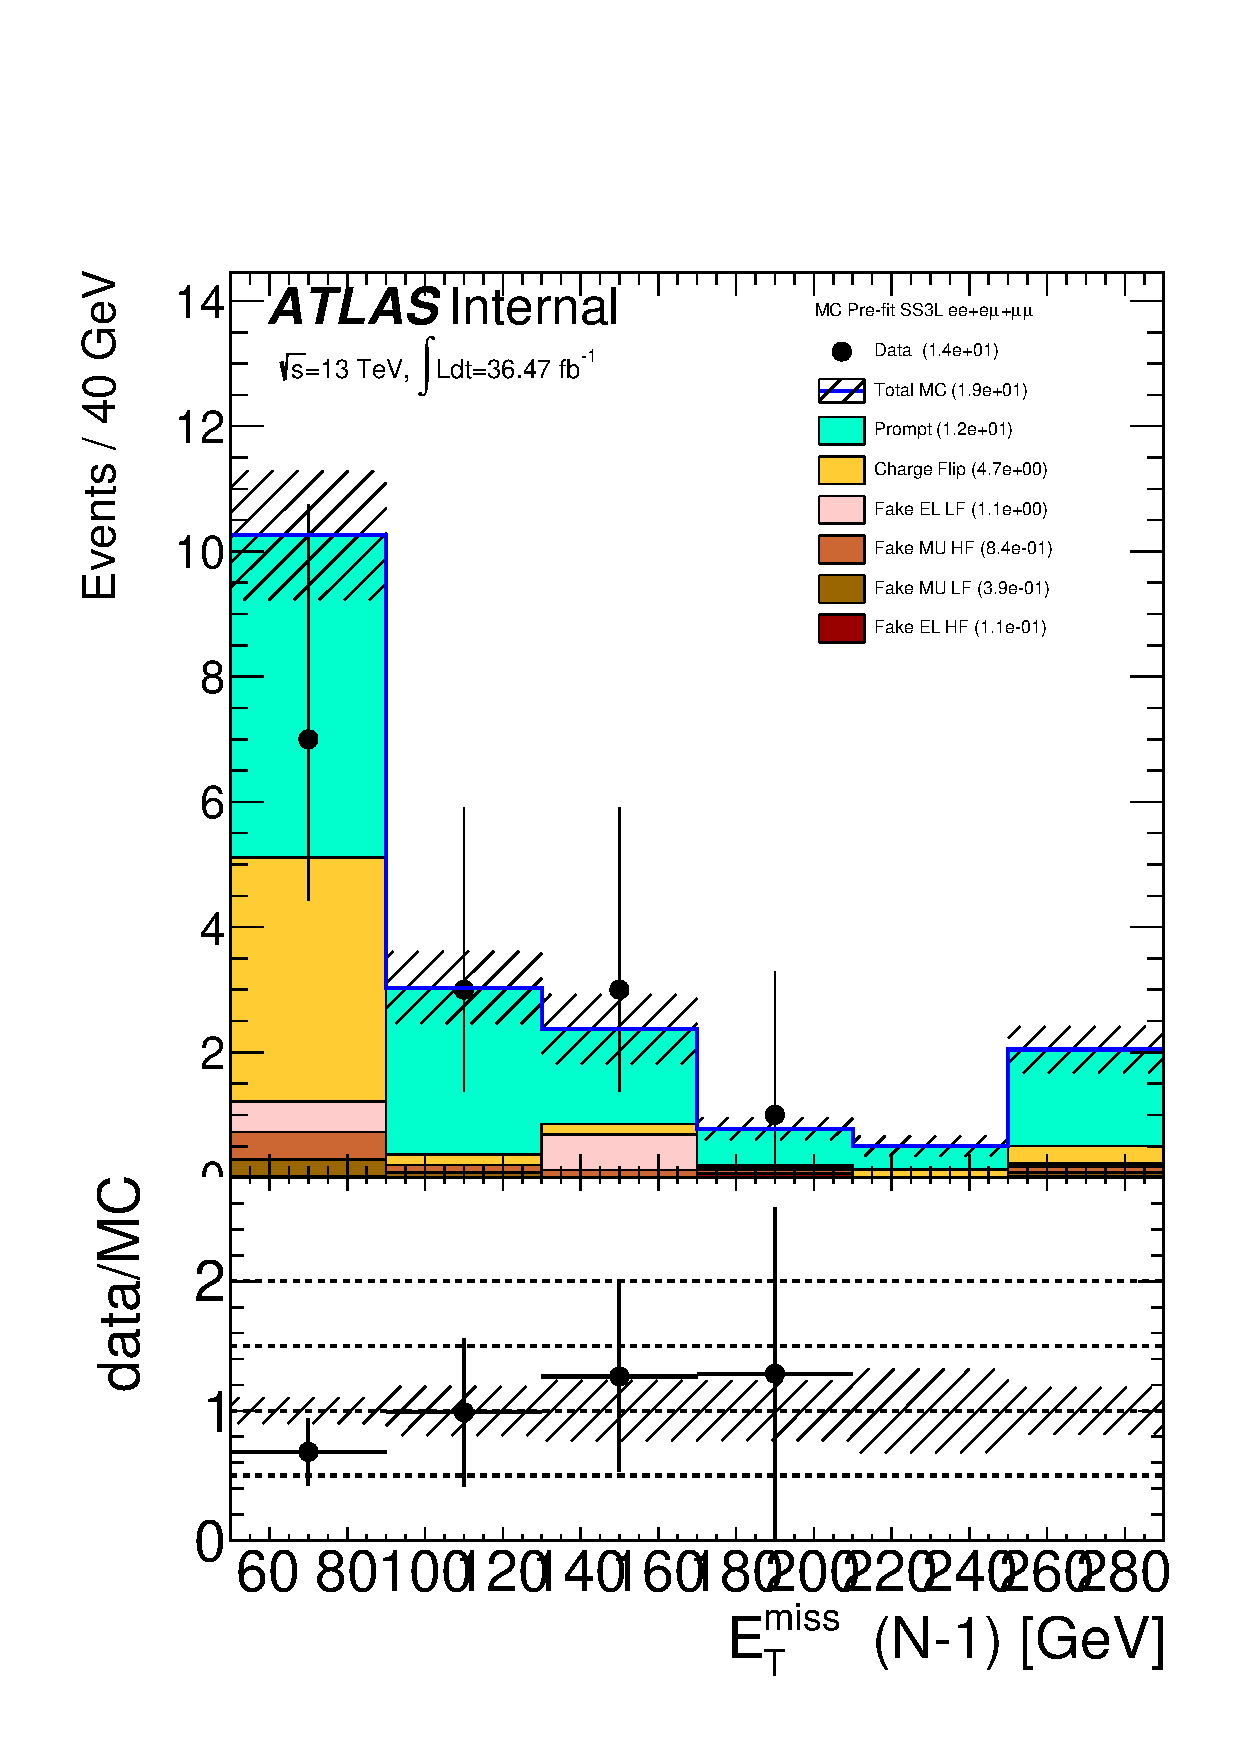
\includegraphics[width=\textwidth]{MET_comb_SR0b2mMET_SS3L.pdf}\caption{}\label{fig:bkg.val.Rpc2L0bH.MCT}\end{subfigure}
\begin{subfigure}[t]{0.49\textwidth}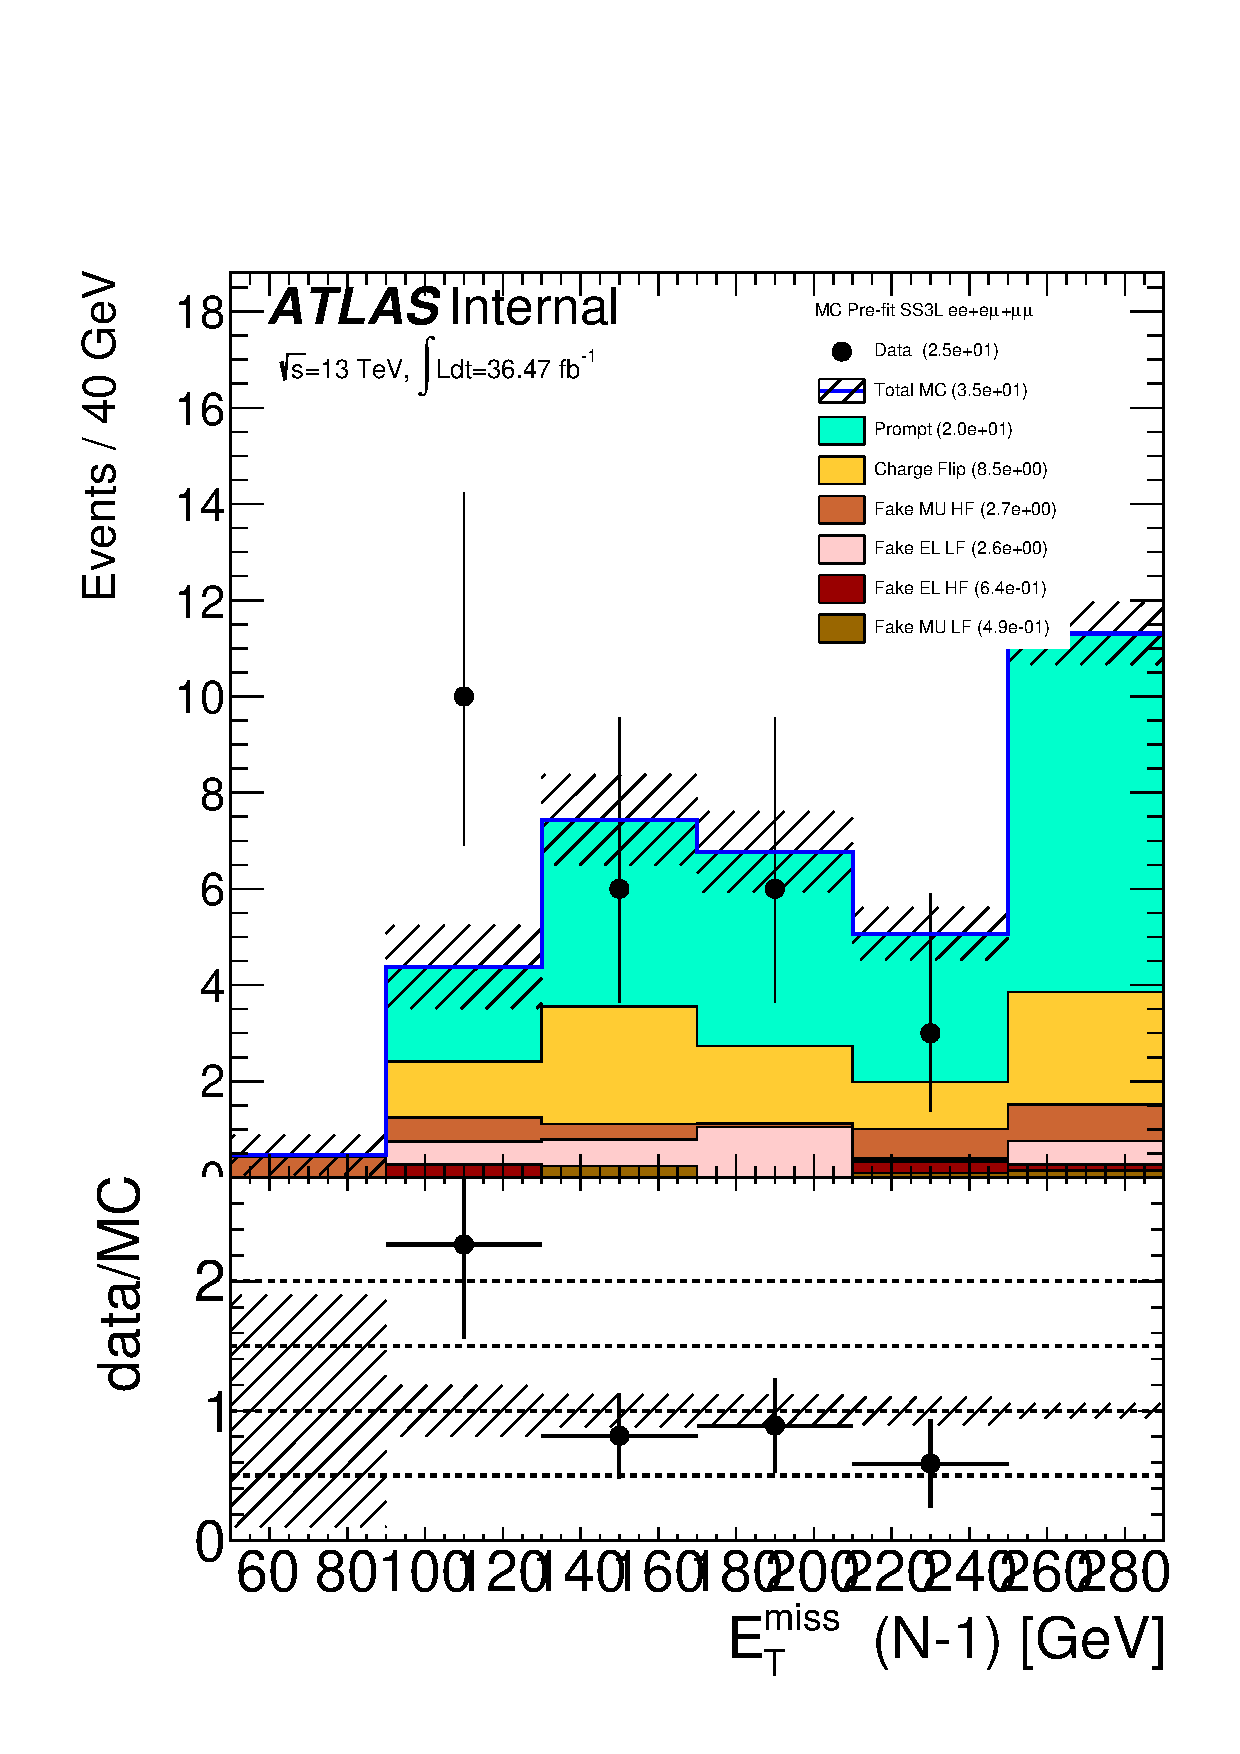
\includegraphics[width=\textwidth]{MET_comb_SR1b2mMET_SS3L.pdf}\caption{}\label{fig:bkg.val.Rpc2L1bH.MCT}\end{subfigure} \\
\caption{
Missing transverse momentum distributions after (\ref{fig:bkg.val.Rpc2L0bH.MxM}--\ref{fig:bkg.val.Rpc2L0bH.MCT}) Rpc2L0bH 
and (\ref{fig:bkg.val.Rpc2L1bH.MxM}--\ref{fig:bkg.val.Rpc2L1bH.MCT}) Rpc2L1bH selection, except the \met~requirement. 
Estimates with the matrix method are in the upper plots (\ref{fig:bkg.val.Rpc2L0bH.MxM}--\ref{fig:bkg.val.Rpc2L0bH.MxM})
while estimates with the MC template method are in the lower plots (\ref{fig:bkg.val.Rpc2L0bH.MCT}--\ref{fig:bkg.val.Rpc2L0bH.MCT}).
The results in the signal regions are shown in the last (inclusive) bin of each plot. 
The statistical uncertainties in the background prediction are included in the uncertainty
band, as well as the full systematic uncertainties for backgrounds with fake or non-prompt leptons, or charge-flip.
}
\label{fig:bkg.val.met}
\end{figure}


\subsection*{Reducible background estimates}

The expected yield for processes with FNP leptons and charge-flip electrons, 
estimated with the matrix method, likelihood method (charge-flip), and the MC template method 
are presented in Table~\ref{tab:fakes_sr_yields} and Table~\ref{tab:chflips_sr_yields} for the signal regions and Table~\ref{tab:VR_Comparison} for the validation regions. 
Since the predictions from the MC template and matrix methods in the signal and validation regions are consistent 
with each other, 
the final numbers retained for the FNP lepton background estimate (also shown in the tables) 
are taken as the weighted-average of the predictions from the matrix method and the MC template; 
the weights are based on the statistical component, and the systematic uncertainties are propagated 
assuming conservatively a full correlation between the two methods (although they are in fact largely independent!). 
The central value and statistical/systematic uncertainties are therefore: 

%\begin{align}
\begin{equation}
\begin{aligned}
\left(w\zeta_1 + (1-w)\zeta_2\right) 
& \pm \sqrt{w^2\left(\Delta\zeta_1^\text{(stat)}\right)^2 + (1-w)^2\left(\Delta\zeta_2^\text{(stat)}\right)^2} \\
& \pm \left(w\Delta\zeta_1^\text{(syst)} + (1-w)\Delta\zeta_2^\text{(syst)}\right)
\end{aligned}
\end{equation}
%\end{align}

$$\qquad\text{ with }w=\frac{\left(\Delta\zeta_2^\text{(stat)}\right)^2}{\left(\Delta\zeta_1^\text{(stat)}\right)^2+\left(\Delta\zeta_2^\text{(stat)}\right)^2}\notag$$

When the estimated value is too small(below 0.15), the expected yield is set to $0.15\pm 0.15$, 
to cover for possibilities of an under-fluctuation of the number of baseline-not-signal leptons 
when applying the matrix method, as well as lack of statistics in the MC samples for the other method. 

The charge flip background is not combined between the MC template method and the likelihood method due to the very large uncertainty in the MC template estimate.
The OS data has a much larger number of events which makes a precise prediction of this background. The MC template result is used as a cross check.

\begin{table}[!htb]
\caption{Expected yields for background processes with fake leptons,
in the signal regions  shown for 36 \ifb. 
Estimates from the matrix method and the MC template method are shown along with the retained estimates.
Uncertainties include all statistical and systematic sources for the nominal estimate.
}
\label{tab:fakes_sr_yields}
\centering
\resizebox{\textwidth}{!}{
\begin{tabular}{|c||c|c|c||c|}\hline
      Region &              Matrix method   &   Template method   &     Retained estimate  \\\hline
    Rpc2L0bH & $ 0.83 \pm  0.56 \pm  0.74$  &  $1.00 \pm 0.96 \pm 0.81$   &  $ 0.87 \pm  0.48 \pm  0.76$  \\
    Rpc2L0bS & $ 1.51 \pm  0.60 \pm  0.66$  &  $1.68 \pm 1.02 \pm 1.26$  &  $ 1.55 \pm  0.52 \pm  0.81$  \\
    Rpc2L1bH & $ 3.54 \pm  1.62 \pm  3.12$  &  $2.07 \pm 0.63 \pm 1.56$   &  $ 2.26 \pm  0.59 \pm  1.76$  \\
    Rpc2L1bS & $ 2.65 \pm  1.21 \pm  1.89$  &  $02.33 \pm 01.17 \pm 02.10$   &  $ 2.48 \pm  0.84 \pm  2.00$  \\ 
    Rpc2L2bH & $-0.11 \pm  0.11 \pm  0.18$  &  $<0.5$  &  $ 0.15 \pm 0.15 \pm  0.00$  \\
    Rpc2L2bS & $ 1.31 \pm  1.07 \pm  1.65$  &  $0.41 \pm 0.33 \pm 0.45$   &  $ 0.49 \pm  0.32 \pm  0.55$  \\
    Rpc2Lsoft1b & $ 4.75 \pm  1.42 \pm  2.64$  &  $2.48 \pm 1.32 \pm 1.86$  &  $ 3.53 \pm  0.97 \pm  2.22$  \\
    Rpc2Lsoft2b & $ 1.91 \pm  1.18 \pm  1.63$  &  $1.66 \pm 0.66 \pm 1.28$  &  $ 1.72 \pm  0.58 \pm  1.36$  \\
    Rpc3L0bH & $-0.01 \pm  0.11 \pm  0.10$  &  $<0.5$  &  $ 0.15 \pm  0.15 \pm  0.00$  \\
    Rpc3L0bS & $ 2.31 \pm  1.50 \pm  2.63$  &  $0.21 \pm 0.15 \pm 0.16$  &  $ 0.23 \pm  0.15 \pm  0.18$  \\
    Rpc3L1bH & $ 0.57 \pm  0.43 \pm  0.50$  &  $0.42 \pm 0.29 \pm 0.32$  &  $ 0.47 \pm  0.24 \pm  0.38$  \\
    Rpc3L1bS & $ 4.94 \pm  1.83 \pm  2.96$  &  $3.55 \pm 1.80 \pm 2.76$  &  $ 4.23 \pm  1.28 \pm  2.86$  \\
    Rpc3LSS1b & $-0.18 \pm  1.24 \pm  2.85$  &  $0.90 \pm 0.14 \pm 0.69$  &  $ 0.89 \pm  0.14 \pm  0.72$  \\
\hline
\hline
\end{tabular}
}
\end{table}

\begin{table}[!htb]
\caption{Expected yields for background processes with charge-flipped electrons,
in the signal regions shown for 36 \ifb. 
Estimates from the likelihood method and the MC template method are shown.
Uncertainties include all statistical and systematic sources. 
Charge-flip processes do not contribute to signal regions which require $\ge 3$ leptons. 
}
\label{tab:chflips_sr_yields}
\centering
\begin{tabular}{|c||c|c|}\hline
 Region      &   Weighted OS data          &     Template method \\\hline
    Rpc2L0bH & $ 0.01 \pm  0.00 \pm  0.00$ & $<0.4$ \\
    Rpc2L0bS & $ 0.05 \pm  0.01 \pm  0.01$ & $ 00.02 \pm 00.02 \pm 00.00 $ \\
    Rpc2L1bH & $ 0.25 \pm  0.03 \pm  0.04$ & $ 00.21 \pm 00.32 \pm 00.16 $ \\
    Rpc2L1bS & $ 0.25 \pm  0.02 \pm  0.04$ & $ 00.35 \pm 00.37 \pm 00.26 $ \\
    Rpc2L2bH & $ 0.02 \pm  0.01 \pm  0.00$ & $<0.4$ \\
    Rpc2L2bS & $ 0.10 \pm  0.01 \pm  0.02$ & $<0.4$ \\
 Rpc2Lsoft1b & $ 0.08 \pm  0.01 \pm  0.02$ & $<0.4$ \\
 Rpc2Lsoft2b & $ 0.08 \pm  0.01 \pm  0.02$ & $<0.4$ \\
   Rpc3LSS1b & $ 0.39 \pm  0.03 \pm  0.07$ & $ 00.81 \pm 00.53 \pm 00.34 $ \\
\hline
\hline
\end{tabular}
\end{table}


\begin{table}[!htb]
\caption{Comparison of expected yields for background processes with fake leptons,
in the validation regions, shown for 36 \ifb~between the data driven (DD) estimates and the MC template method (MC) estimates. 
}
\label{tab:VR_Comparison}
\def\arraystretch{1.1}
\centering
\resizebox{0.8\textwidth}{!}{
\begin{tabular}{|c|c|c|c|c|c|}
\hline 
               & VR-$t\bar t W$ & VR-$t\bar t Z$ & VR-$WZ$4j & VR-$WZ$5j & VR-$W^\pm W^{\pm}$  \\\hline	   
Fakes DD       & $23 \pm 5 \pm 24$      & $30 \pm 4 \pm 14$   & $53 \pm 6 \pm 27$   & $21 \pm 4 \pm 10$  & $14 \pm 3 \pm 10$ \\
Fakes MC       & $14 \pm 4 \pm 10$      & $18 \pm 3 \pm 13 $  & $46 \pm 5  \pm 34$  & $16 \pm 2 \pm 12$  & $13 \pm 2 \pm 10$ \\\hline
Combined       & $18 \pm 3 \pm 15$      & $22 \pm 2 \pm 13$   & $49 \pm 4 \pm 30$   & $17 \pm 2 \pm 12$  & $13 \pm 2 \pm 10$ \\\hline
Charge-flip DD & $3.4 \pm 0.1 \pm 0.5$  & $-$                 & $-$                 & $-$                & $1.7 \pm 0.1\pm 0.2$ \\
Charge-flip MC & $3.8  \pm 1.0 \pm 1.9$ & $-$                 & $-$                 & $-$                & $1.0 \pm 0.3 \pm 0.2$\\
\hline
\end{tabular}}
\end{table}
